\documentclass{book}
\usepackage{titling}
\usepackage{multirow}
\usepackage{setspace}
\usepackage{makeidx}
\usepackage{tikz}
\usepackage{braket}
\usepackage{graphicx}
\usepackage{array}

\usepackage{qcircuit}
\usepackage{graphicx}

\usepackage{tabularray}
\usepackage{amsmath}
\usepackage{circuitikz}
\usepackage{amssymb}
\usepackage{setspace}
\usepackage{amsmath}
\usepackage{xepersian}
\settextfont{XB Zar}
\linespread{1.5}



\makeatletter
\def\TikzBipolePath#1#2{\pgf@circ@bipole@path{#1}{#2}}
\def\CircDirection{\pgf@circ@direction}
\makeatother

% TikZ libraries `calc` needed now to tweak bracket.
\usetikzlibrary{backgrounds,fit,decorations.pathreplacing,calc}

\begin{document}
\tableofcontents
\section{مقدمه}	
در عصر حاضر بواسطه‌ی رشد و توسعه‌ی نظریه‌ی اطلاعات کوانتومی و سرمایه‌گذاری های مالی و انسانی بسیار در این زمینه،‌شاهد افزایش تعداد علاقمندان به این حوزه هستیم. در این پا .....

\section{comp vs superpos basis}
Consider the circuit shown in Figure 1.17, which applies Uf to an input not in the
computational basis. Instead, the data register is prepared in the superposition (|0〉 +
|1〉)/√2, which can be created with a Hadamard gate acting on |0〉. Then we apply Uf ,
resulting in the state:
% https://g.co/bard/share/2972a6a63b24



\chapter{آشنایی با مفاهیم اولیه}
\section{کیوبیت}

یک کیوبیت\footnote{Qubit}، معادل یک واحد اطلاعات کوانتومی می‌باشد. این مفهوم معادل مفهوم کلاسیک بیت\footnote{Binary Bit} می‌باشد. به طور کلی هر کیوبیت حاوی دو بیت اطلاعات است. برای تبیین یک کیوبیت از خصوصیات سامانه های کوانتومی، بهره‌می‌بریم. کیوبیت یک سیستم کوانتومی با فضای دوبعدی است. برای تعیین این دوبعد می‌توان ا ز یکی از خصویات سامانه های کوانتومی استفاده کرد. 

برخلاف بیت ها که مقادیر ثابت 0 یا 1 را به خود می‌گیرند؛ یک کیوبیت می‌تواند در یک حالت «برهمنهی کوانتومی» باشد؛ این بدان معناست که یک کیوبیت بواسطه‌ی مشاهده ناظر به یکی از حالات 0 یا یک تبدیل شود. این مهم‌ترین مزیت استفاده از کیوبیت‌هاست. بیان ریاضی یک کیوبیت ،در حالت برهمنهی، به شرح زیر است:
\vspace{2cm}
$$
\left\{
\begin{array}{ll}
	  \vert \psi \rangle = \alpha\vert 0 \rangle + \beta\vert 1 \rangle \\
	  \alpha^2 + \beta^2 = 1
\end{array}
\right.
$$
\vspace{2cm}

\newpage
کت‌ها$\vert 0 \rangle$ و $\vert 1 \rangle$ بیانگر پایه‌های فضای 
محاسباتی\footnote{\lr{Computational Basis Vectors}} هستند؛ و مقادیر $\alpha^2$ و $\beta^2$ بیانگر احتمال وقوع هر یک از این حالات، در صورت مشاهده، می‌باشند.

نمایش بردار $\psi$ به شرح زیر است:
\begin{center}
\begin{tikzpicture}
	
	% Define the axes
	\draw[->] (-2,0)--(2,0) node[right]{$\vert 0 \rangle$};
	\draw[->] (0,-2)--(0,2) node[above]{$\vert 1 \rangle$};
	
	% Draw the vector
	\draw[black,-stealth] (0,0)--(1,2) node[anchor=south west]{$\vec{\psi}$};
	
	% Label the components of the vector
	\node[below] at (1,0) {$$};
	\node[left] at (0,2) {$$};
	
\end{tikzpicture}
\end{center}

در بسیاری از مواقع برای سهولت در محاسبات، عملگر‌ها و حالات کوانتومی به کمک ماتریس‌ها نمایش داده ‌می‌شوند. فرم ماتریسی هر یک از حالات ذکر شده در بالا به شرح زیر است:

\begin{equation}
	\vert 1 \rangle = \begin{pmatrix} 0 \\ 1 \end{pmatrix}
	\hspace{2cm}
	\vert 0 \rangle = \begin{pmatrix} 1 \\ 0 \end{pmatrix}	
\end{equation}

برای تعریف کیوبیت ها، راه های زیادی وجود دارد، حالات قطبش فوتون،‌اسپین الکترون،‌یا سطوح انرژی اتم،‌هریک می‌توانند تعیین کننده‌ی بردار‌های فضای کیوبیت باشند.

\section{bloch vector - computayional basis - fourier basis}
\section{گیت‌های کوانتومی}
گیت‌های کوانتومی\footnote{\lr{Quantum Gates}} یکی از اولین و ههم‌ترین اجزای‌ مدار‌های کوانتومی ‌می‌باشند. این گیت‌ها عملگر‌هایی با قابلیت اثر‌گذاری روی کیوبیت‌ها می‌باشند. با اعمال یک گیت کوانتومی بر روی یک یا چند کیوبیت، می‌توان تغییرات مدنظر خود را روی کیوبیت اعمال کرد. با کمک این گیت‌ها می‌توان باعث برهم‌نهی کوانتومی یا رمز‌گذاری داده در داخل یک یا چند کیوبیت شد.

\subsection{انواع گیت کوانتومی}
گیت‌های کوانتومی، دارای انواع مختلف گوناگونی می‌باشند. به طور کلی گیت‌های کوانتومی، عملگر‌هایی یکه و بازگشت‌پذیر می‌باشند. 
\subsection*{گیت هادامارد}
مهم‌ترین گیت کوانتومی،‌گیت هادامارد\footnote{\lr{Hadamard gate}} است. با اعمال اثر این گیت روی یک کیوبیت، آن کیوبیت به‌یک حالت برهم نهی‌ کوانتومی‌ گذار‌ می‌کند. به عبارت دیگر هر یک از زیرحالات این حالت برهم‌نهی، با احتمال یکسانی قابل رخ دادن‌ هستند. 
\vspace{1cm}
$$
H\ket{0} = \frac{1}{\sqrt{2}} (\ket{0} + \ket{1})
\hspace{2cm}
H\ket{1} = \frac{1}{\sqrt{2}} (\ket{0} - \ket{1})
$$
\vspace{1cm}

این گیت کوانتومی‌ به صورت خطی روی یک دسته‌ کت اثر مي‌کند. نمایش ماتریسی این گیت‌کوانتومی به شرح زیر است:
\begin{center}
	\[
	H = \frac{1}{\sqrt{2}}
	\begin{pmatrix}
		1 & 1 \\
		1 & -1
	\end{pmatrix}
	\]
\end{center}





\begin{align*}
	H |0\rangle = l\frac{1}{\sqrt{2}} \begin{pmatrix} 1 & 1 \\ 1 & -1 \end{pmatrix} \begin{pmatrix} 1 \\ 0 \end{pmatrix} \
	= \frac{1}{\sqrt{2}} \begin{pmatrix} 1 \\ 1 \end{pmatrix} \
	= \frac{1}{\sqrt{2}} (|0\rangle + |1\rangle)
\end{align*}

\begin{align*}
	H |1\rangle = l\frac{1}{\sqrt{2}} \begin{pmatrix} 1 & 1 \\ 1 & -1 \end{pmatrix} \begin{pmatrix} 0 \\ 1 \end{pmatrix} \
	= \frac{1}{\sqrt{2}} \begin{pmatrix} 1 \\ -1 \end{pmatrix} \
	= \frac{1}{\sqrt{2}} (|0\rangle - |1\rangle)
\end{align*}

این گیت کوانتومی، یک گیت بازگشت‌پذیر است؛ یعنی اگر این گیت روی یک حالت کوانتومی اثر کند؛‌ می‌تواند آن را از حالت برهمنهی خارج کند. 

برای اعمال این گیت کوانتومی، فقط به یک کیوبیت نیاز داریم. به اصطلاح این گیت،‌یک \lr{Single-Qubit Quantum gate} می‌باشد.

نمایش این گیت‌کوانتومی در مدار با علامت زیر است:
\Qcircuit @C=1em @R=1.2em {
	& & \qw & \gate{H} & \qw \\
	& & & & \\
}


\subsection*{گیت CNOT}

گیت کوانتومی \lr{CNOT}\footnote{ controlled-NOT gate or controlled-X gate}، به عنوان گیت منطقی، یاد می‌شود. این گیت کوانتومی معادل گیت \lr{NOT} کلاسیک می‌باشد.
به‌طور معمول، برای اعمال اثر این گیت کوانتومی نیاز به دو کیوبیت داریم. این گیت کوانتومی فقط و فقط در مواقعی که «کیوبیت کنترل\footnote{Controled Qubit}» دارای مقدار $\vert 1 \rangle$ باشد، باعث تغییر وضعیت «کیوبیت هدف\footnote{Target Qubit}» می‌شود.

کیوبیت کنترل:
کیوبیت هدف:

خلاصه‌ای از عملکرد این تابع به شرح زیر است:\\
\textbf{ببین چرا از این نماد به جای تنسور پراداکت استفاده شده}
\begin{latin}
\begin{tabular}{ccccc}
	&&&&\\
	|A & B$\rangle$ &	&  |A &B $\oplus$ A $\rangle$  \\
	|control$\rangle$ & |target$\rangle$ & Effect CNOT Gate &|control$\rangle$ & |target$\rangle$ \\
	------- & -------- & -------- & -------- & --------  \\
	|0$\rangle$ & |0$\rangle$ & $\Longrightarrow$ &|0$\rangle$ & |0$\rangle$ \\
	|0$\rangle$ & |1$\rangle$ & $\Longrightarrow$ &|0$\rangle$ & |1$\rangle$ \\
	|1$\rangle$ & |0$\rangle$ & $\Longrightarrow$ &|1$\rangle$ & |0$\rangle$ \\
	|1$\rangle$ & |1$\rangle$ & $\Longrightarrow$ &|1$\rangle$ & |1$\rangle$
\end{tabular}
\end{latin}



نمایش ماتریسی این گیت کوانتومی به شکل زیر است:



اینا باید اصلاح بشه

$$
\text{CNOT} = \begin{pmatrix}
	1 & 0 & 0 & 0 \\
	0 & 1 & 0 & 0 \\
	0 & 0 & 0 & 1 \\
	0 & 0 & 1 & 0
\end{pmatrix}
$$



$$
\text{CNOT} \ket{1} = \begin{pmatrix}
	1 & 0 & 0 & 0 \\
	0 & 1 & 0 & 0 \\
	0 & 0 & 0 & 1 \\
	0 & 0 & 1 & 0
\end{pmatrix} \begin{pmatrix}
	1 \\
	0 \\
	0 \\
	0
\end{pmatrix} = \begin{pmatrix}
	0 \\
	0 \\
	0 \\
	1
\end{pmatrix} = \ket{1}
$$


$$
\text{CNOT} \ket{11} = \begin{pmatrix}
	1 & 0 & 0 & 0 \\
	0 & 1 & 0 & 0 \\
	0 & 0 & 0 & 1 \\
	0 & 0 & 1 & 0
\end{pmatrix} \begin{pmatrix}
	1 \\
	1 \\
	0 \\
	0
\end{pmatrix} = \begin{pmatrix}
	0 \\
	1 \\
	0 \\
	0
\end{pmatrix} = \ket{10}
$$
\vspace{2cm}

نمایش در داخل مدار:

\vspace{2cm}
\Qcircuit @C=1em @R=.7em {
	& \ctrl{1} & \targ & \qw \\
	& \targ & \ctrl{-1} & \qw
}

از این گیت کوانتومی‌، برای بسیاری مدار‌ها و شبیه‌سازی‌های کوانتومی، از جمله تلپورت، درهمتنیدگی و ...، استفاده می‌شود.





\subsubsection*{گیت توفولی}
گیت کوانتومی توفولی،‌یک نوع خاص از گیت \lr{CNOT} است. سازوکار این گیت مشابه گیت \lr{CNOT} می‌‌باشد؛‌ با این تفاوت که با در نظر گرفتن وضعیت دو کیوبیت کنترل شده، وضعیت کیوبیت سوم را تغییر می‌دهد. خلاصه ای از عملکرد این گیت کوانتومی به شرح زیراست:

به بیان دیگر اگر دو کیوبیت کنترل شده،‌ مقدار یک داشته باشند؛‌ کیوبیت هدف مقدارش تغییر می‌کند.
فرم ماتریسی این عملگر به شکل زیر است:

این گیت کوانتومی در مدار کوانتومی به شکل زیر نشان داده می‌شود:

\subsection*{گیت تغییر فاز}
گیت تغییر فاز\footnote{Phase shift gate}، یکی از گیت های مهم کوانتومی‌ می‌باشد. این گیت با ضرب کردن یک عدد ثابت در فاز یک کیوبیت، باعث تغییر فاز کیوبیت می‌شود. این گیت کوانتومی در بسیاری از الگوریتم‌های سرچ کوانتومی به‌کار می‌رود. این گیت بدین صورت تعریف می‌شود:

فرم ماتریسی این گیت به شرح زیر است:

این گیت کوانتومی در مدار کوانتومی به شکل زیر نشان داده می‌شود:

\subsection*{گیت دوران}
گیت دوران، \footnote{Rotation gate}، باعث دوران حالت کیوبیت، در فضای هیلبرت ‌می‌شود. پایه‌های فضای هیلبرت مذکور بردار های................................... هستند. نمایش این گیت کوانتومی به شرح زیر است:

فرم ماتریسی این گیت به شرح زیر است:
نمایش این گیت در مدار کوانتومی به شرح زیراست:


\subsection{Swap gate}

% https://www.youtube.com/watch?v=_p7i2v21Ys8&t=188s
% https://www.youtube.com/watch?v=F2okky5vD8k&list=PL1826E60FD05B44E4&index=11



\section{مدار‌های کوانتومی}

مدار‌های ‌کوانتومی\footnote{quantum circuit}، یک دسته از گیت ها‌ی کوانتومی،که با یک توالی بخصوص قرار گرفته اند، ‌می‌باشند. این کیوبیت ها، با توالی یاد شده، روی یک یا چند دسته کیوبیت، اثر داده ‌می‌شوند. 

مدار‌های کوانتومی، یکی از اولین مفهوم‌های بکار‌رفته برای تعریف کامپیوتر‌های کوانتومی‌ می‌باشند. برای تعریف و شبیه‌سازی هریک از پدیده‌ها و الگوریتم‌های کوانتومی، نیاز به یک مدار به‌خصوص داریم.

\subsubsection{شباهت ها و تفاوت های مدارهای کلاسیک و کوانتومی}
Quantum circuits are similar to classical circuits, but they use quantum gates instead of classical logic gates. Quantum gates are reversible operations that can be used to manipulate the quantum state of a qubit.

Sure, here are some similarities and differences between quantum circuits and classical circuits:

**Similarities:**

* Both quantum and classical circuits are composed of a sequence of operations that are applied to a set of data.
* Both circuits can be represented graphically using a similar notation.
* Both circuits can be used to implement algorithms.

**Differences:**

* Quantum circuits use qubits, which are quantum bits, as their basic unit of data. Classical circuits use bits, which are classical bits, as their basic unit of data.
* Quantum circuits use quantum gates, which are reversible operations, as their basic operations. Classical circuits use logic gates, which are irreversible operations, as their basic operations.
* Quantum circuits can exploit the properties of quantum mechanics, such as superposition and entanglement, to perform tasks that are impossible for classical computers.

Here is a table that summarizes the similarities and differences between quantum circuits and classical circuits:

| Feature | Quantum Circuit | Classical Circuit |
|---|---|---|
| Basic unit of data | Qubit | Bit |
| Basic operations | Quantum gates | Logic gates |
| Reversibility | Reversible | Irreversible |
| Exploits quantum mechanics | Yes | No |
| Possible tasks | Factoring integers, searching unsorted databases, simulating quantum systems | Sorting, calculating, logical operations |

I hope this helps! Let me know if you have any other questions.


\subsubsection{اجزای مدار‌های کوانتومی و سایز آن }
Operations: Operations are the actions that are performed on qubits. They can be measurements, initializations, or other actions.


The size of a quantum circuit is the number of gates in the circuit. The complexity of a quantum algorithm is often measured in terms of the size of the quantum circuit that is required to implement it.


Qubits

Qubits are the basic unit of information in quantum computing. They can be in a superposition of two states, 0 and 1. This means that a qubit can be both 0 and 1 at the same time, which is a property called quantum superposition. Qubits can also be entangled, which means that the state of one qubit is dependent on the state of another qubit.

Gates

Gates are operations that are applied to qubits. They can be used to create superpositions, perform rotations, and entangle qubits. There are many different types of gates, but some of the most common ones include the Hadamard gate, the CNOT gate, and the Toffoli gate.

Operations

Operations are the actions that are performed on qubits. They can be measurements, initializations, or other actions. Measurements are used to collapse the quantum state of a qubit into a definite value, 0 or 1. Initializations are used to set the state of a qubit to a specific value, 0 or 1.

Quantum Circuits

Quantum circuits are written using a graphical notation that is similar to the circuit diagrams used in classical computing. The horizontal axis of a quantum circuit represents time, and the vertical axis represents the qubits. The gates are represented by boxes, and the lines between the boxes represent the connections between the qubits.

Conclusion

The basic components of a quantum circuit are qubits, gates, and operations. These components are used to create quantum algorithms, which are algorithms that can only be performed on a quantum computer. Quantum circuits are a powerful tool for quantum computation, and they have the potential to revolutionize many different fields, including cryptography, chemistry, and machine learning.


\subsection{نحوه‌ی نمایش مدار‌های کوانتومی}

Quantum circuits are written using a graphical notation that is similar to the circuit diagrams used in classical computing. The horizontal axis of a quantum circuit represents time, and the vertical axis represents the qubits. The gates are represented by boxes, and the lines between the boxes represent the connections between the qubits.

Quantum circuits are a powerful tool for quantum computation. They can be used to implement a wide variety of quantum algorithms, including Shor's algorithm for factoring integers and Grover's algorithm for searching unsorted databases.

\chapter{برنامه‌نویسی کوانتومی}
\section{تفاوت کامپیوتر کلاسیک و کوانتومی}
\section{IBM Quantum computer and Qiskit}

\chapter{الگوریتم‌های‌کوانتومی‌}


چه گونه‌ای از مسائل محاسباتی قابل اجرا با مدارهای کوانتومی می‌باشند؟ 
تفاوت و برتری مدار‌های کوانتومی نسبت به مدار‌های کلاسیک چیست؟
آیا می‌توان یک حوزه‌ی خاص را تعیین کرد؛ به گونه‌ای که عملکرد کامپیوترهای‌‌کوانتومی نسبت به کامپیوتر‌های کلاسیک مزیت داشته باشند؟

در این بخش می‌خواهیم به طور خلاصه این سوالات را پاسخ دهیم و توضیح دهیم چگونه می‌توان از کامپیوتر‌های کوانتومی به شکلی سودمند استفاده کنیم.

\section{موازی سازی کوانتومی}

موازی‌سازی کوانتومی\footnote{Quantum parallelism}، پایه‌واساس بسیاری از الگوریتم‌های کوانتومی است. با گذار یک حالت کوانتومی به حالت برهمنهی کوانتومی، درحین محاسبات کوانتومی یک تابع نظیر \lr{f(x)}، می‌تواند مقادیر مختلف \lr{x} را به طور همزمان بررسی کند. این درحالیست که در محاسبات کلاسیک به دلیل ماهیت بیت‌های اطلاعات، تابع \lr{f(x)} فقط می‌تواند یکی از مقادیر مجاز برای \lr{x} را بررسی کند.


فرض کنید تابع f ،یک تابع تک-کیوبیت، به صورت زیر تعریف شده است:\\
\begin{center}
	$f (x) : \{0, 1\} \rightarrow \{0, 1\}$\\
\end{center}

روش مناسب برای محاسبه این تابع در یک کامپیوتر کوانتومی، با در نظر گرفتن دو کیوبیت که در حالت $\vert x, y\rangle$شروع می شود. با یک توالی مناسب از گیت های منطقی می توان این حالت را به $\vert f(x) \oplus x, y\rangle$ تبدیل کرد که در آن $\oplus$ بیانگر جمع مدوله با پایه‌2 می‌باشد.

\footnote{Modulo 2 is a mathematical operation that returns the remainder of a division by 2. For example, 5 mod 2 is 1, because 5 divided by 2 has a quotient of 2 and a remainder of 1.
	
	The symbol "⊕" is often used to indicate addition modulo 2. So, the expression "5 ⊕ 3" would be evaluated as follows:
	
	5 ⊕ 3 = (5 + 3) mod 2 = 8 mod 2 = 0
	This is because 8 divided by 2 has a quotient of 4 and a remainder of 0.
	
	Modulo 2 is a useful operation in many different areas of mathematics, including cryptography, computer science, and number theory. It is also used in everyday life, for example, when checking whether a number is even or odd.
	
	Here are some other examples of modulo 2:
	
	1 mod 2 = 1
	2 mod 2 = 0
	3 mod 2 = 1
	4 mod 2 = 0
	5 mod 2 = 1}

هریک از دسته‌های کیوبیت، \textbf{رجیستر کوانتومی} نامیده‌می‌شوند. اولین رجیستر، «رجیستر داده» و دومین رجیستر «رجیستر هدف» نامیده می‌شود.\\
ازین پس در این بخش به عامل گذار $\vert x, y \rangle \rightarrow \vert x, y \oplus f(x) \rangle$، عنوان «تابع \lr{$U_{f}$}» را اطلاق خواهیم کرد. لازم به ذکرست که این تبدیل، یک تبدیل یکه به شمار می‌آید.\footnote{اثبات این مطلب از حوصله‌ی بحث خارج است.}


اگر \lr{y = 0} آنگاه مقدار دومین کیوبیت بعد از اعمال تابع \lr{$U_{f}$} برابر با مقدار \lr{f(x)} خواهد بود.

 \begin{center}
 	 \begin{figure}[ht]
 		\centering
 		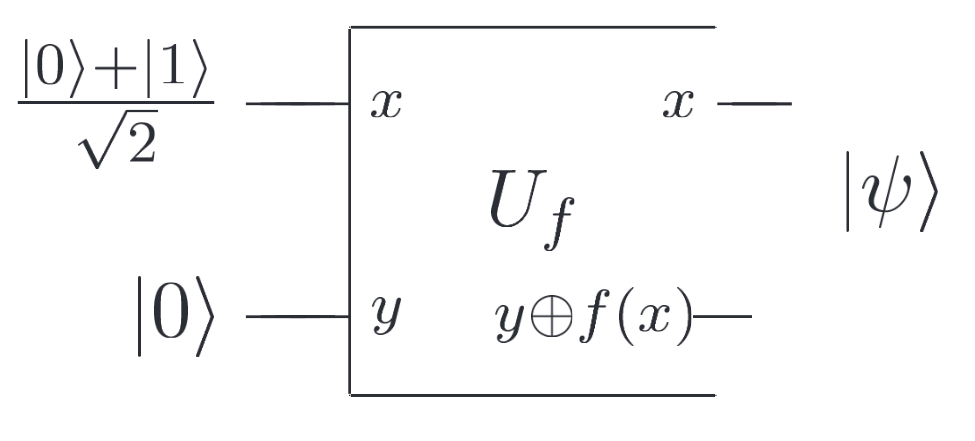
\includegraphics[width=0.8\textwidth]{Uforacle.png}
 		\caption{مدار کوانتومی برای ارزیابی $f (0)$ و $f (1)$ به طور همزمان. Uf مدار کوانتومی است که ورودی هایی مانند $\vert x, y\rangle$ را به $\vert x, y \rangle \rightarrow \vert x, y \oplus f(x) \rangle$، تصویر می‌کند.}
 	\end{figure}
 \end{center}

در شکل بالا مقادیر ورودی داده شده به تابع \lr{$U_{f}$} در پایه‌های محاسباتی قرار ندارند. رجیستر داده در حالت برهمنهی  قرار دارد. این حالت برهمنهی را می‌توان با اعمال گیت هادامارد بر حالت کوانتومی $\vert 0 \rangle$ ایجاد کرد. پس از ایجاد این حالت، تابع \lr{$U_{f}$} را به حالت جدید اعمال می‌کنیم:
\begin{center}
	$\frac{\vert 0,f(0) \rangle +\vert 1,f(1) \rangle }{\sqrt{2}}$
\end{center}

این یک حالت استثنایی است! جملات مختلف کسر بالا حاوی اطلاعاتی در مورد f (0) وf (1) می‌باشند؛ به‌نحوی که انگار f (x) را برای دو مقدار x به طور همزمان ارزیابی کرده ایم، این ویژگی به "موازی  سازی کوانتومی" موسوم می‌باشد. بر خلاف موازی سازی کلاسیک، که در آن هر یک مدارهای متعددی دارند ساخته شده برای محاسبه f (x) به طور همزمان اجرا می شوند، در اینجا برای ارزیابی تابع برای چندین مقدار x به طور همزمان، یک مدار f (x) (با قابلیت برهمنهی کوانتومی)استفاده می شود.

این فرآیند را می توان به راحتی  با استفاده از یک عمل کلی به نام تبدیل هادامارد، به توابعی با تعداد بیت دلخواه تعمیم داد. این عمل فقط تعداد n گیت هادامارد است که به طور موازی روی n کوبیت عمل می کنند.



 For example, shown in Figure 1.18 is the case n = 2 with qubits initially prepared as |0〉, which gives
( |0〉 + |1〉√2) ( |0〉 + |1〉√2) = |00〉 + |01〉 + |10〉 + |11〉 as output.
2 (1.38)

برای مثال در شکل زیر؛ دو کیوبیت در حالت $\vert 0 \rangle$ آماده شده‌‌اند. پس از اعمال گیت‌های هادامارد بر روی این رجیستر به خروجی زیر خواهیم رسید: 

\begin{center}
	$ \Biggl( \frac{\vert 0 \rangle + \vert 1 \rangle}{\sqrt{2}}\Biggl)\Biggl( \frac{\vert 0 \rangle + \vert 1 \rangle}{\sqrt{2}}\Biggl) = \frac{\textbar00\rangle + \textbar01\rangle + \textbar10\rangle + \textbar11\rangle}{\sqrt{2}}$

\end{center}

از نماد $\operatorname{H} \otimes 2$ به عنوان نشانه‌ی عملکرد موازی دو گیت هادامارد استفاده می‌کنیم؛از علامت $\otimes$ به عنوان تانسور یاد می‌کنیم. به طور کلی نتایج اعمال موازی گیت هادامارد روی \lr{n} کیوبیت روی حالت کوانتومی برابرست با:

\begin{center}
	\[\frac{1}{\sqrt{2}} \sum_{x} \vert x \rangle\]
\end{center}

where the sum is over all possible values of x, and we write H⊗n to denote this action.
That is, the Hadamard transform produces an equal superposition of all computational
basis states. Moreover, it does this extremely efficiently, producing a superposition of 2n
states using just n gates.



Figure 1.18. The Hadamard transform H⊗2 on two qubits.
Quantum parallel evaluation of a function with an n bit input x and 1 bit output, f (x),
can thus be performed in the following manner. Prepare the n + 1 qubit state |0〉⊗n|0〉,
then apply the Hadamard transform to the first n qubits, followed by the quantum circuit
implementing Uf . This produces the state
1
√2n
∑
x
|x〉|f (x)〉 . (1.40)






In some sense, quantum parallelism enables all possible values of the function f to be
evaluated simultaneously, even though we apparently only evaluated f once. However,
this parallelism is not immediately useful. In our single qubit example, measurement of the
state gives only either |0, f (0)〉 or |1, f (1)〉! Similarly, in the general case, measurement of
the state ∑
x |x, f (x)〉 would give only f (x) for a single value of x. Of course, a classical
computer can do this easily! Quantum computation requires something more than just
quantum parallelism to be useful; it requires the ability to extract information about more
than one value of f (x) from superposition states like ∑
x |x, f (x)〉. Over the next two
sections we investigate examples of how this may be done








\newpage
\subsection{مدل محاسباتی استاندارد}
پیش از بررسی مدل کوئری،‌ مدل ساده و استاندارد محاسباتی را بررسی می‌کنیم. به تصویر زیر دقت کنید:

\begin{figure}[ht]
	\centering
	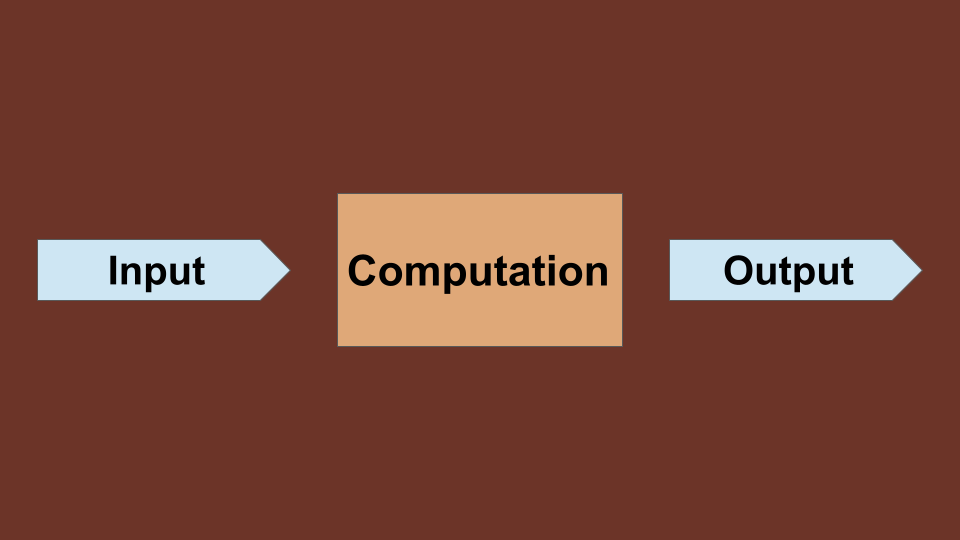
\includegraphics[width=0.8\textwidth]{standard computation model.png}
	\caption{یک واحد محاسباتی که مقادیری را به عنوان ورودی گرفته، پردازش کرده و سپس مقدار/مقادیر خروجی را ارائه کرده است.}
\end{figure}


در تصویر بالا یک نمود ساده از کامپیوتر‌های امروزی ارائه شده است. در دنیای واقعی مقدار ورودی می‌تواند از هر منبعی‌ تأمین شده باشد. با این وجود هدف ما بررسی منابع تولید ورودی نیست؛‌ بلکه هدف بررسی مقادیر ورودی (به صورت ایزوله) می‌باشد. می‌توان درنظر گرفت که ورودی داده شده و خروجی نهایی،‌هر دو در قالب یک رشته از اعداد باینری، ماتریس و یا هرقالب مدنظر کاربر باشند.

مهم‌ترین نکته درباره‌ی این واحد محاسباتی،‌ \textbf{در دسترس بودن کل مقادیر ورودی برای واحد پردازش} است. به عبارت دیگر\textbf{ واحد پردازش می‌تواند تمامی مقادیر ورودی را دریافت کرده و تشخیص} دهد. 

\subsection{مدل کوئری}
در مدل کوئری، داده‌های ورودی توسط یک تابع تولید می‌شوند. واحد محاسباتی دسترسی به تابع تولیدورودی دارد و می‌تواند برای دریافت داده‌های جدید،‌از تابع یاد شده،‌درخواست کند.

\begin{figure}[ht]
	\centering
	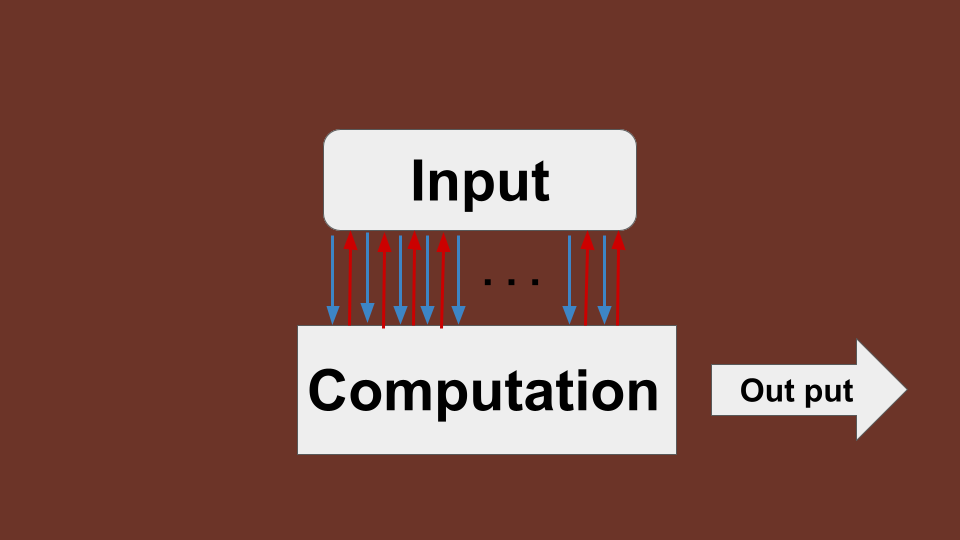
\includegraphics[width=0.8\textwidth]{Query computation model.png}
	\caption{شکل بالا نمود مدل محاسباتی‌کوئری است. واحد محاسباتی برای دریافت داده‌های جدید نیاز به درخواست از تابع \lr{input} دارد. خطوط قرمز و روبه‌بالا نشان از درخواست واحد محاسباتی و خطوط آبی روبه‌پایین نشان از پاسخ واحد \lr{input}می‌باشد.}
\end{figure}


در این مدل واحد محاسباتی دیگر داده‌ها را در قالب رشته‌ای از اطلاعات دردسترس ندارد؛ بلکه می‌تواند آن‌ها را از بخش \lr{input} دریافت کند. در گاهی از مواقع به سیستم \lr{input}،‌\lr{oracle} یا جعبه‌ی سیاه می‌گویند. تابع \lr{Oracle } یا جعبه‌ی سیاه یک سیستم است که ما به عنوان ناظر به سازوکار داخلی آن و  تمامی اطلاعات آن دسترسی نداریم و فقط می‌توانیم مقادیر مجاز را به آن داده و مقادیر خروجی را دریافت کنیم. 

تابع \lr{oracle} به صورت زیر تعریف می‌شود:
\begin{center}
$$
\left\{
\begin{array}{ll}
f : \sum^n = \sum^m\\
Which : m, n \in \mathbb{N}
\end{array}
\right.
$$
\end{center}

ما در این نظریه کوئری‌ها را می‌شماریم و وضعیت آن‌‌ها را بررسی می‌کنیم.

\section*{الگوریتم‌های کوانتومی}


%https://learn.qiskit.org/course/algorithms/query-algorithms#query-3-0
%https://www.youtube.com/watch?v=mGqyzZ-fnnY
%https://www.youtube.com/watch?v=CIq0PUkFDBc
%https://www.youtube.com/watch?v=7MdEHsRZxvo
%https://learn.qiskit.org/course/algorithms/query-algorithms#query-3-77
%https://learn.qiskit.org/course/algorithms/query-algorithms#query-5-0
%https://learn.qiskit.org/course/algorithms/query-algorithms#query-19-0
%https://www.youtube.com/watch?v=hK6BBluTGhU&list=PLay4zC7VCXV4gWb0ucSUQiGcRJFYMzROT&index=5
	
\section{Deutsch Algorithm}
tell combnation of books
\subsection{مسئله‌ی دوچ}
الگوریتم \lr{Deutsch} اولین و ساده‌ترین الگوریتم کوانتومی‌ است. این الگوریتم برای اولین بار در سال 1985 در مقاله‌ای مطرح شد؛ که توسط دیوید دوچ\footnote{David Deutsch} نوشته شده‌‌بود. این الگوریتم نقطه‌ی شروعی برای اثبات برتری کامپیوترهای کوانتومی نسبت به کامپوترهای کلاسیک است.

مسئله‌ی \lr{Deutsch} یکی از ساده‌ترین مفاهیم ممکن را مطرح می‌کند. اگر یک تابع به فرم زیر تعریف شود: 
\begin{center}
	$f : \sum \rightarrow \sum$
\end{center}
هدف بررسی ثابت بودن یا متعادل\footnote{Constante or balanse.} بودن تابع \lr{f} است. 
به‌طور کلی، درساده‌ترین حالت، می‌توان چهار وضعیت را برای تابع $f : \sum \rightarrow \sum$ درنظر گرفت:\\
\begin{figure}[ht]
	\centering
	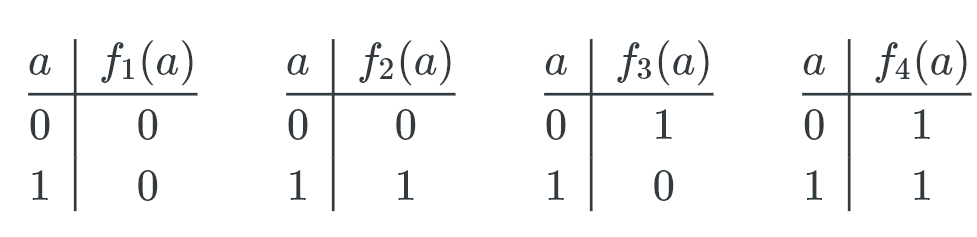
\includegraphics[width=0.8\textwidth]{Constantorbalanse.png}
	\caption{}
\end{figure}\\
در شکل بالا توابع \lr{f 1} , \lr{f 4} توابع ثابت و توابع \lr{f 2} و \lr{f 3} توابع متعادل هستند.
\begin{center}
\begin{tabular}{|c|c|}
	\hline
	\multicolumn{2}{|c|}{مسئله‌ی دوچ} \\
	\hline
	$f : \sum \rightarrow \sum$ & ورودی \\
	\hline
	صفر اگر تابع ثابت بود؛ یک اگر تابع متعادل بود.  & خروجی \\
	\hline
\end{tabular}
\end{center}
در الگوریتم‌های کلاسیک برای حل این مسئله، حداقل دو حالت باید بررسی شود.
\subsection{الگوریتم دوچ}
% https://www.youtube.com/watch?v=2wticzHE1vs&t=2014s
% page 32

حال به بررسی الگوریتم دوچ می‌پردازیم. الگوریتمی که مسئله‌ی دوچ را با یک مدار کوانتومی حل می‌کند:\\
\begin{center}
\begin{figure}[ht]
	\centering
	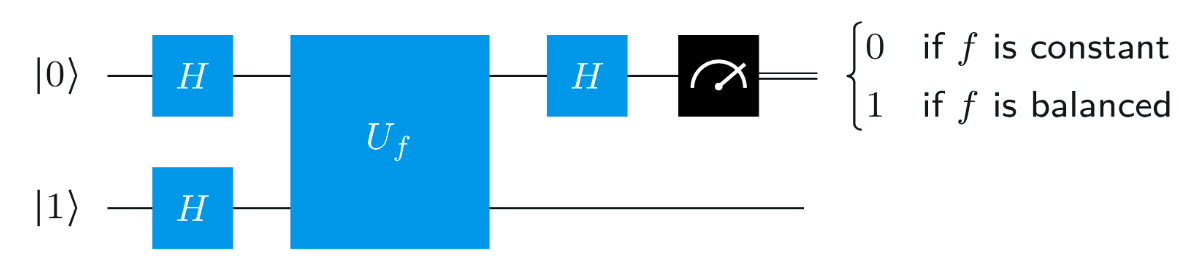
\includegraphics[width=0.8\textwidth]{Deutsch algorithm.png}
	\caption{}
\end{figure}
\end{center}


$$
\begin{aligned}
	\left|\pi_1\right\rangle= & |-\rangle|+\rangle=\frac{1}{2}(|0\rangle-|1\rangle)|0\rangle+\frac{1}{2}(|0\rangle-|1\rangle)|1\rangle \\
	\left|\pi_2\right\rangle= & \frac{1}{2}(|0 \oplus f(0)\rangle-|1 \oplus f(0)\rangle)|0\rangle+\frac{1}{2}(|0 \oplus f(1)\rangle-|1 \oplus f(1)\rangle)|1\rangle \\
	= & \frac{1}{2}(-1)^{f(0)}(|0\rangle-|1\rangle)|0\rangle+\frac{1}{2}(-1)^{f(1)}(|0\rangle-|1\rangle)|1\rangle \\
	& |0 \oplus a\rangle-|1 \oplus a\rangle=(-1)^a(|0\rangle-|1\rangle)
\end{aligned}
$$

$$
\begin{aligned}
	\left|\pi_1\right\rangle & =|-\rangle|+\rangle=\frac{1}{2}(|0\rangle-|1\rangle)|0\rangle+\frac{1}{2}(|0\rangle-|1\rangle)|1\rangle \\
	\left|\pi_2\right\rangle & =\frac{1}{2}(|0 \oplus f(0)\rangle-|1 \oplus f(0)\rangle)|0\rangle+\frac{1}{2}(|0 \oplus f(1)\rangle-|1 \oplus f(1)\rangle)|1\rangle \\
	& =\frac{1}{2}(-1)^{f(0)}(|0\rangle-|1\rangle)|0\rangle+\frac{1}{2}(-1)^{f(1)}(|0\rangle-|1\rangle)|1\rangle \\
	& =|-\rangle\left(\frac{(-1)^{f(0)}|0\rangle+(-1)^{f(1)}|1\rangle}{\sqrt{2}}\right)
\end{aligned}
$$

$$
\begin{aligned}
	\left|\pi_2\right\rangle & =|-\rangle\left(\frac{(-1)^{f(0)}|0\rangle+(-1)^{f(1)}|1\rangle}{\sqrt{2}}\right) \\
	& =(-1)^{f(0)}|-\rangle\left(\frac{|0\rangle+(-1)^{f(0) \oplus f(1)}|1\rangle}{\sqrt{2}}\right) \\
	& = \begin{cases}(-1)^{f(0)}|-\rangle|+\rangle & f(0) \oplus f(1)=0 \\
		(-1)^{f(0)}|-\rangle|-\rangle & f(0) \oplus f(1)=1\end{cases}
\end{aligned}
$$


$$
\begin{aligned}
	\left|\pi_2\right\rangle & = \begin{cases}(-1)^{f(0)}|-\rangle|+\rangle & f(0) \oplus f(1)=0 \\
		(-1)^{f(0)}|-\rangle|-\rangle & f(0) \oplus f(1)=1\end{cases} \\
	\left|\pi_3\right\rangle & = \begin{cases}(-1)^{f(0)}|-\rangle|0\rangle & f(0) \oplus f(1)=0 \\
		(-1)^{f(0)}|-\rangle|1\rangle & f(0) \oplus f(1)=1\end{cases} \\
	& =(-1)^{f(0)}|-\rangle|f(0) \oplus f(1)\rangle
\end{aligned}
$$

$$
\left|\pi_3\right\rangle=(-1)^{f(0)}|-\rangle|f(0) \oplus f(1)\rangle
$$
توضیحات رو بنویس



\newpage

\section{Deutsch-Jozsa Algorithm}




% https://www.youtube.com/watch?v=DyINHZoOcLQ
%https://www.youtube.com/watch?v=LTftC-eTLM0SS
--------------	
	
	
	
%computer vs simulator https://www.youtube.com/watch?v=2qcvgXaDdfU
% https://www.youtube.com/watch?v=0RPFWZj7Jm0	
	
\section{oracle}
use qiskit site
\chapter{شبیه‌سازی پدیده‌های کوانتومی}
\section{Bell states}
% pls search about bell eq
در این بخش قصد داریم به بررسی پروتکل‌های ابتدایی در نظریه‌ی اطلاعات کوانتومی بپردازیم. تمامی این پروتکل‌ها به تعداد کمی کیوبیت نیاز دارند:؛ و در آزمایشگاه به صورت تجربی پیاده‌سازی شده‌اند. در اغلب موارد، سیستم از دو کیوبیت درهمتنیده تشکیل شده‌است. تابع حالت این سیستم‌ها به شکل زیر تعریف می‌شوند:
\begin{center}
	$\vert \psi_{00} \rangle = \frac{1}{\sqrt{2}}(|00\rangle + |11\rangle)$
\end{center}
برای آماده‌سازی این حالت کوانتومی‌، در حالت \lr{$\vert0\rangle$} داریم. با اعمال یک گیت هدامارد روی یکی از کیوبیت‌ها و سپس با کنترل‌ آن با گیت \lr{CNOT}، (به نحوی که کیوبیت دوم هدف قرارگیرد.) می‌توان به یک حالت درهمتنیده رسید. می‌توان این مراحل را به شکل زیر شرح داد:
\begin{center}
	$\vert\psi_{00}\rangle = C_{10}H_{1}\vert00\rangle$
\end{center}

%می‌توان رابطه‌ی بالا را به هریک از حالات $\vert00\rangle, \vert 01\rangl, \vert 10\rangl, \vert 11\rangl$ تعمیم داد:%
\[
\vert\psi_{xy}\rangle = C_{10}H_{1}\vert xy \rangle
\]

از آنجایی که چهار حالت |xy〉 یک مجموعه orthonormal هستند و دروازه‌های Hadamard و cNOT واحدی هستند، چهار حالت درهم تنیده |ψxy〉 نیز یک مجموعه orthonormal هستند، که به نام پایه Bell نامگذاری شده‌اند. حال یک دسته‌ی سه‌کیوبیتی را درنظر ‌می‌گیریم:

% read about bell state equation
\begin{center}
$\vert \psi_{xy}\rangle = C10H1X^{x}_{1} X^{y}_{0} \vert00\rangle$\\
\end{center}

last paragraph of page 136 of quantum computer scince book??\\
\section{entanglement}
\section{super dense coding}
quntum computer scinse
\section{Teleport}
isac book
فرض کنید آلیس یک کیوبیت در حالت زیر دارد:
\begin{center}
$\vert \psi \rangle = \alpha\vert 0 \rangle + \beta\vert 1 \rangle $\\	
\end{center}

	کارول ممکن است با اعمال یک عملگر یکه‌ به یک کیوبیت در حالت استاندارد، کیوبیت را از حالت $\vert0\rangle$ به حالت $\vert\psi\rangle$  تبدیل کرده باشد. کارول بدون اعلام نوع عملگر یکه به آلیس،‌ کیوبیت را برای او ارسال می‌کند. 
	حال آلیس می‌خواهد بدون دسترسی داشتن به کیوبیت باب، تغییراتی را در کیوبیت او ایجاد کند؛ این تنها درصورتی ممکن است که کیوبیت باب و آلیس درهمتنیده باشند. هرچند آلیس و باب می‌توانند از طریق راه‌های کلاسیک(نظیر تلفنی صحبت کردن و ...) با یکدیگر ارتباط برقرار کنند؛ ولی نمی‌توانند دسترسی مستقیم به کیوبیت یکدیگر داشته باشند. 
	
	کیوبیت باب را می‌توان به حالت زیر تعریف کرد:
$\vert\phi\rangle = 1/\sqrt{2}(\vert0\rangle \vert0\rangle + \vert1\rangle\vert1\rangle)$ 
	

==============
اکنون تکنیک های چند صفحه آخر را برای درک چیزی غیرمعمول به کار خواهیم برد.
پیش پا افتاده، غافلگیر کننده و بسیار سرگرم کننده - دوربری کوانتومی! تله پورت کوانتومی یک است
تکنیک حرکت حالات کوانتومی به اطراف، حتی در غیاب ارتباط کوانتومی
کانال nications که فرستنده حالت کوانتومی را به گیرنده پیوند می دهد.
در اینجا نحوه عملکرد دوربری کوانتومی آمده است. آلیس و باب مدت ها پیش با هم آشنا شدند اما اکنون زندگی می کنند
دور از هم. در حالی که آنها با هم یک جفت EPR تولید کردند که هر کدام یک کیوبیت از EPR را می گرفتند
وقتی از هم جدا شدند جفت شوند سال‌ها بعد، باب مخفی است و ماموریت آلیس باید انجام شود
او تصمیم می گیرد آن را بپذیرد، یعنی یک کیوبیت |ψ〉 به باب تحویل دهد. او وضعیت را نمی داند
کیوبیت، و علاوه بر این فقط می تواند اطلاعات کلاسیک را برای باب ارسال کند. آیا آلیس باید قبول کند
ماموریت؟
به طور شهودی، همه چیز برای آلیس بسیار بد به نظر می رسد. او وضعیت |ψ〉 آن را نمی داند
کیوبیت او باید برای باب بفرستد و قوانین مکانیک کوانتومی او را از این کار باز می دارد
تعیین وضعیت زمانی که او فقط یک نسخه از |ψ〉 در اختیار دارد. چه
بدتر از آن، حتی اگر او حالت |ψ〉 را می دانست، توصیف دقیق آن به مقدار بی نهایت نیاز دارد.
اطلاعات کلاسیک از آنجایی که |ψ〉 مقادیر را در یک فضای پیوسته می گیرد. بنابراین حتی اگر او انجام دهد
بدانید |ψ〉، همیشه طول می کشد تا آلیس وضعیت را برای باب توصیف کند. نگاه نمی کند
برای آلیس خوبه خوشبختانه برای آلیس، انتقال از راه دور کوانتومی راهی برای استفاده از آن است
جفت EPR درهم به منظور ارسال |ψ〉 به باب، تنها با سربار کوچک کلاسیک
ارتباط
به طور کلی، مراحل حل به شرح زیر است: آلیس با کیوبیت |ψ〉 با
نصف او از جفت EPR، و سپس دو کیوبیت در اختیارش را اندازه گیری می کند و به دست می آورد
یکی از چهار نتیجه کلاسیک ممکن، 00، 01، 10، و 11. او این اطلاعات را به
باب بسته به پیام کلاسیک آلیس، باب یکی از چهار عمل خود را انجام می دهد
نیمی از جفت EPR. به طرز شگفت انگیزی، با انجام این کار او می تواند حالت اولیه را بازیابی کند |ψ〉!
مدار کوانتومی نشان داده شده در شکل 1.13 توصیف دقیق تری از کوانتوم ارائه می دهد
دوربری حالتی که باید از راه دور منتقل شود عبارت است از |ψ〉 = α|0〉+β|1〉 که α و β ناشناخته هستند.
دامنه ها حالت ورودی مدار |ψ0〉 است
|ψ0〉 = |ψ〉|β00〉





 1
√2
[
α|0〉(|00〉 + |11〉) + β|1〉(|00〉 + |11〉)
]
, (1.29
\\

که در آن از این قرارداد استفاده می کنیم که دو کیوبیت اول (در سمت چپ) متعلق به آلیس هستند و
کیوبیت سوم به باب. همانطور که قبلا توضیح دادیم، کیوبیت دوم آلیس و کیوبیت باب
در حالت EPR شروع کنید. آلیس کیوبیت های خود را از طریق دروازه می فرستد و به دست می آورد
|ψ1〉 = 1
√2
[
α|0〉(|00〉 + |11〉) + β|1〉(|10〉 + |01〉)
]
. (1.30)
سپس اولین کیوبیت را از طریق دروازه هادامارد می فرستد و به دست می آورد
|ψ2〉 = 1
2
[
α(|0〉 + |1〉)(|00〉 + |11〉) + β(|0〉− |1〉)(|10〉 + |01〉)
]
.
(1.31)
این حالت را می توان به روش زیر بازنویسی کرد، به سادگی با گروه بندی مجدد عبارات:
|ψ2〉 = 1
2
[
|00〉 (α|0〉 + β|1〉) + |01〉 (α|1〉 + β|0〉)
+ |10〉 (α|0〉 − β|1〉) + |11〉 (α|1〉− β|0〉)]
. (1.32)
این عبارت به طور طبیعی به چهار اصطلاح تقسیم می شود. عبارت اول دارای کیوبیت های آلیس است
در حالت |00〉 و کیوبیت باب در حالت α|0〉 + β|1〉 - که حالت اصلی است.
|ψ〉. اگر آلیس یک اندازه گیری را انجام دهد و نتیجه 00 را به دست آورد، سیستم باب این کار را انجام می دهد
در حالت بودن |ψ〉. به طور مشابه، از عبارت قبلی می‌توانیم پست باب را بخوانیم
حالت اندازه گیری، با توجه به نتیجه اندازه گیری آلیس:
00 −→ |ψ3 (00)〉 ≡
[
α|0〉 + β|1〉
]
(1.33)
01 −→ |ψ3 (01)〉 ≡
[
α|1 + β|0»
]
(1.34)
10 −→ |ψ3 (10)〉 ≡
[
α|0〉 − β|1〉
]
(1.35)
11 −→ |ψ3 (11)〉 ≡
[
α|1〉− β|0〉
]
. (1.36)
بسته به نتیجه اندازه گیری آلیس، کیوبیت باب به یکی از این موارد ختم می شود
چهار حالت ممکن البته برای اینکه بدانیم در کدام حالت است باید نتیجه را به باب گفت
اندازه گیری آلیس - بعداً نشان خواهیم داد که این واقعیت است که از دوربری جلوگیری می کند




رام برای انتقال اطلاعات سریعتر از نور استفاده می شود. وقتی باب این معنی را یاد گرفت
در نتیجه، باب می‌تواند وضعیت خود را «تثبیت» کند، و با استفاده از روش مناسب |ψ〉 بهبود یابد.
دروازه کوانتومی به عنوان مثال، در موردی که اندازه گیری 00 را به دست می آورد، باب این کار را نمی کند
نیاز به انجام هر کاری اگر اندازه گیری 01 باشد، باب می تواند با اعمال کردن حالت خود را اصلاح کند
دروازه X اگر اندازه گیری 10 باشد، باب می تواند وضعیت خود را با اعمال Z ثابت کند
دروازه. اگر اندازه‌گیری 11 باشد، باب می‌تواند با اعمال ابتدا یک X و حالت خود را اصلاح کند
سپس یک دروازه Z. به طور خلاصه، باب باید تبدیل ZM1 XM2 را اعمال کند (به چگونگی آن توجه کنید
زمان در نمودارهای مداری از چپ به راست می‌رود، اما در سمت راست در محصولات ماتریسی می‌رود
اول اتفاق می افتد) به کیوبیت او، و او حالت |ψ〉 را بازیابی می کند.
بسیاری از ویژگی های جالب تله پورت وجود دارد که به برخی از آنها اشاره خواهیم کرد
به بعد در کتاب. در حال حاضر به اظهار نظر در مورد چند مورد بسنده می کنیم
جنبه های. اولا، آیا تله‌پورتاسیون به فرد اجازه نمی‌دهد حالت‌های کوانتومی را سریع‌تر از آن ارسال کند
سبک؟ این امر نسبتاً عجیب و غریب خواهد بود، زیرا نظریه نسبیت نشان می دهد که سریعتر
از انتقال اطلاعات نور می توان برای ارسال اطلاعات به عقب در زمان استفاده کرد.
خوشبختانه، تله‌پورت کوانتومی امکان ارتباط سریع‌تر از نور را فراهم نمی‌کند.
زیرا برای تکمیل دوربری، آلیس باید نتیجه اندازه گیری خود را به آن ارسال کند
باب از طریق یک کانال ارتباطی کلاسیک.


ما در بخش 2.4.3 نشان خواهیم داد که بدون این ارتباط کلاسیک، از راه دور هیچ اطلاعاتی را منتقل نمی کند. کانال کلاسیک با سرعت نور محدود می شود، بنابراین نتیجه می شود که تله پورت کوانتومی نمی تواند سریعتر از سرعت نور انجام شود و پارادوکس ظاهری را حل کند. معمای دوم در مورد تلهپورتاسیون این است که به نظر می رسد یک کپی از حالت کوانتومی در حال انتقال از راه دور ایجاد می کند، که آشکارا قضیه عدم شبیه سازی مورد بحث در بخش 1.3.5 را نقض می کند. این نقض فقط توهمی است زیرا پس از فرآیند انتقال از راه دور فقط کیوبیت هدف در حالت |ψ〉 باقی می ماند و کیوبیت داده اصلی بسته به نتیجه اندازه گیری به یکی از حالت های پایه محاسباتی |0 یا |1 می رسد. در کیوبیت اول از تله پورت کوانتومی چه چیزی می توانیم یاد بگیریم؟ خیلی زیاد! این خیلی بیشتر از یک ترفند ساده است که می توان با حالت های کوانتومی انجام داد. تله پورت کوانتومی بر قابلیت تعویض منابع مختلف در مکانیک کوانتومی تاکید می کند و نشان می دهد که یک جفت EPR مشترک به همراه دو بیت کلاسیک ارتباط، منبعی حداقل برابر با یک کیوبیت ارتباط است. محاسبات کوانتومی و اطلاعات کوانتومی روش‌های زیادی را برای تبادل منابع نشان داده‌اند که بسیاری از آنها بر اساس تله‌پورت کوانتومی ساخته شده‌اند. به طور خاص، در فصل 10 توضیح می دهیم که چگونه می توان از تله پورت برای ساخت دروازه های کوانتومی مقاوم در برابر اثرات نویز استفاده کرد و در فصل 12 نشان دادیم که انتقال از راه دور با ویژگی های کدهای تصحیح خطای کوانتومی ارتباط نزدیکی دارد. علیرغم این ارتباط با موضوعات دیگر، منصفانه است که بگوییم که ما تازه در حال درک این موضوع هستیم که چرا انتقال از راه دور کوانتومی در مکانیک کوانتومی امکان پذیر است. در فصل‌های بعدی سعی می‌کنیم برخی از بینش‌هایی را توضیح دهیم که چنین درکی را ممکن می‌سازد. 1

\newpage
how to determine a oracle\\
	
	
	
	
% https://learn.qiskit.org/course/ch-algorithms/quantum-circuits
	
	
	
\end{document}